\documentclass[landscape]{article}

%\usepackage[top=0.4in,bottom=0.4in,left=0.75in,right=0.5in]{geometry}
\usepackage[paperwidth=13.13636in,paperheight=8.5in,top=0.4in,bottom=0.3in,left=0.75in,right=0.75in]{geometry}  % aspect ratio same as 11x17 (1.5454)
\usepackage{graphicx}
\usepackage{caption}
\usepackage{subcaption}
\usepackage{nopageno}
\pagestyle{plain}
\usepackage{array}
\usepackage[export]{adjustbox}
\usepackage{tabularx} % table features
\usepackage{booktabs} % table features
\usepackage[abs]{overpic} % overlaying one graphic on another
\usepackage{xstring,xifthen} % string length with conditionals
\usepackage{color} % colored text
\usepackage{helvet} % font
%\usepackage{cmbright} % font
%\usepackage{avant} % font

\DeclareGraphicsExtensions{.pdf}

\renewcommand{\familydefault}{\sfdefault}

\parindent=0pt
\baselineskip=0pt
\parskip=0pt

\input{macros.tex}

%%%%%%%%%% BEGIN DOCUMENT / HEADER %%%%%%%%%%

\begin{document}

%\begin{tabularx}{\textwidth}{ X c X }     %<--does better with horizontal spacing
\begin{tabular}{ m{4.4cm} m{16cm} }  %<--does better with vertical spacing
	~~
\includegraphics[height=0.08\textheight]{statics/logoshape.pdf} & 
\includegraphics[height=0.065\textheight]{statics/youramericangutsampletext.pdf} \\
\end{tabular}

\hrule

\vspace{0.65cm}

%%%%%%%%%% NAME %%%%%%%%%%

\begin{center}

\StrLen{\yourname}[\yournameLen]

\ifthenelse{\yournameLen < 28}{
	{\fontfamily{phv}\fontsize{38}{48}\selectfont {\MakeUppercase {\bf \yourname}}}
}{
	{\fontfamily{phv}\fontsize{34}{46}\selectfont {\MakeUppercase {\bf \yourname}}}
}

\end{center}

\vspace{0.65cm}

%%%%%%%%%% FIRST ROW %%%%%%%%%%

{\huge What's in your \sampletype{} sample?}

\vspace{2mm}

\begin{tabular*}{\textwidth}{ m{0.3in} m{4.0in} m{7.5in} }
	&
	\vspace{2mm}
	\hspace{-5mm}
	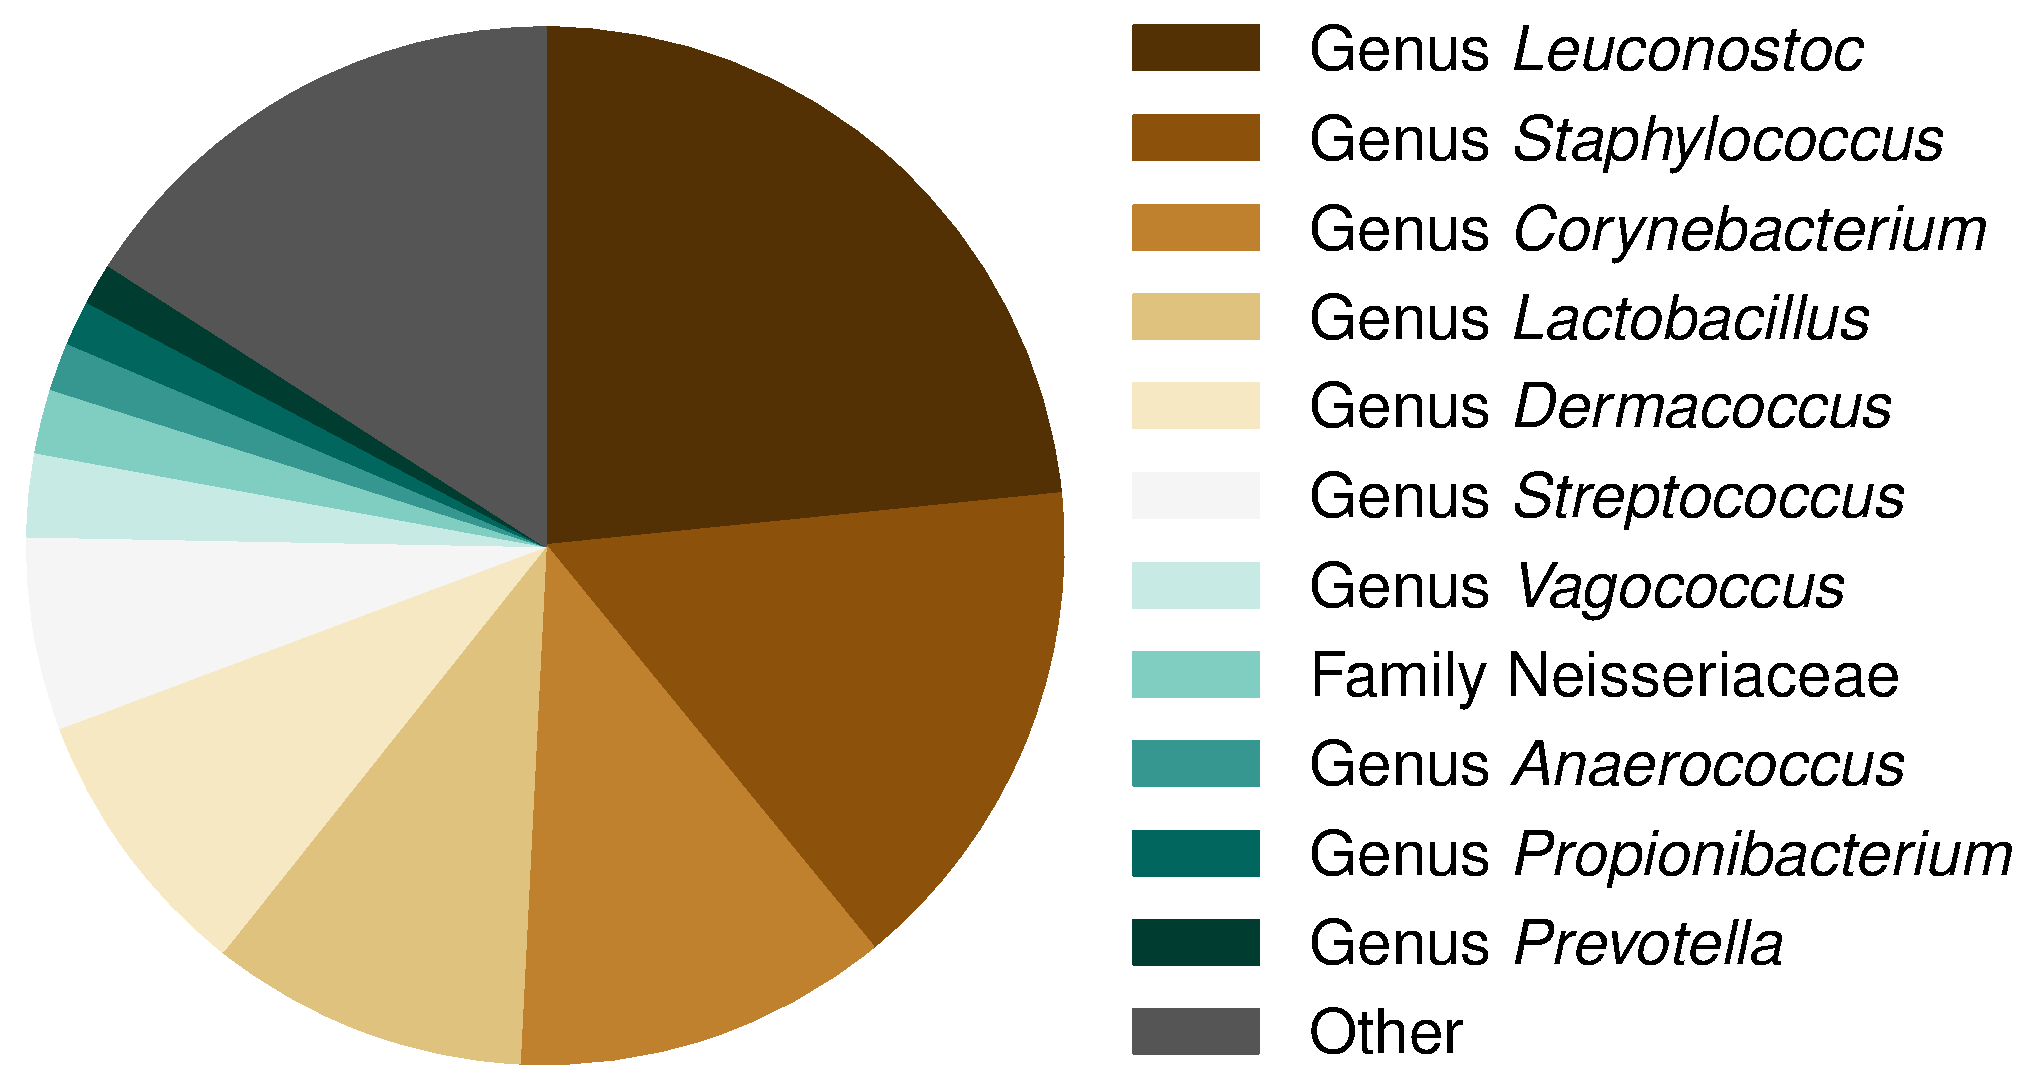
\includegraphics[scale=0.27]{figure2.pdf}
	
    &
    {\normalsize 
    \vspace{2.5mm}
    \parbox[b][][t]{6.5in}{
	\begin{tabular}{ c l r c l r r r }
    \multicolumn{3}{l}{\large ~~Your most abundant microbes:} & \multicolumn{5}{l}{\large ~~Your most enriched microbes:}\\ \addlinespace[2mm]
        \cline{2-3} \cline{5-8} \addlinespace[1mm]
        & Taxonomy & Sample & & Taxonomy & Sample & Population & Fold \\
        \cline{2-3} \cline{5-8} \addlinespace[1mm]
        & \abundTaxonA{} & \abundSamplA{}\% & & \enrichTaxonA{} & \enrichSamplA{}\% & \enrichPopulA{}\% & \enrichFoldA{}x \\
        & \abundTaxonB{} & \abundSamplB{}\% & & \enrichTaxonB{} & \enrichSamplB{}\% & \enrichPopulB{}\% & \enrichFoldB{}x \\
        & \abundTaxonC{} & \abundSamplC{}\% & & \enrichTaxonC{} & \enrichSamplC{}\% & \enrichPopulC{}\% & \enrichFoldC{}x \\
        & \abundTaxonD{} & \abundSamplD{}\% & & \enrichTaxonD{} & \enrichSamplD{}\% & \enrichPopulD{}\% & \enrichFoldD{}x \\
        \cline{2-3} \cline{5-8} \addlinespace[3mm]
        & \multicolumn{7}{p{5.6in}}{\footnotesize \rareList{}} \\
        & \multicolumn{7}{p{5.6in}}{\footnotesize This sample was registered on \sampledate{} at \sampletime{}.}
	\end{tabular}
	}
	}
\end{tabular*}

\vspace{5mm}

%%%%%%%%%% SECOND ROW %%%%%%%%%%

{\huge How do your \sampletype{} microbes compare to others?} \hspace{1cm} 
\includegraphics[scale=0.45]{pdfs-gut/ball_legend.pdf}

\vspace{5mm}

\begin{tabular*}{\textwidth}{ m{3.5in} m{3.7in} m{3.7in} }

\vspace{-10mm}
\begin{overpic}[width=2.10in]{figure4.pdf}
	\ifthenelse{\equal{\sampletype}{oral}}{\put(-32,-42){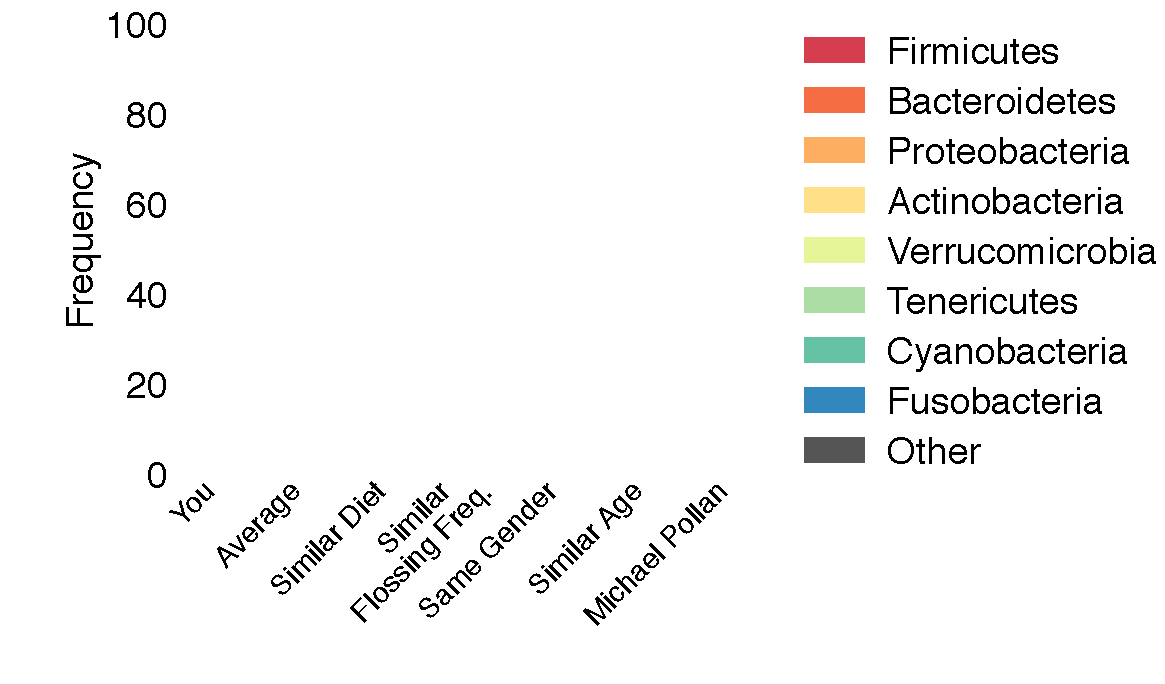
\includegraphics[width=3.65in]{statics/barchart_overlay_oral.pdf}}}{}
	\ifthenelse{\equal{\sampletype}{skin}}{\put(-32,-42){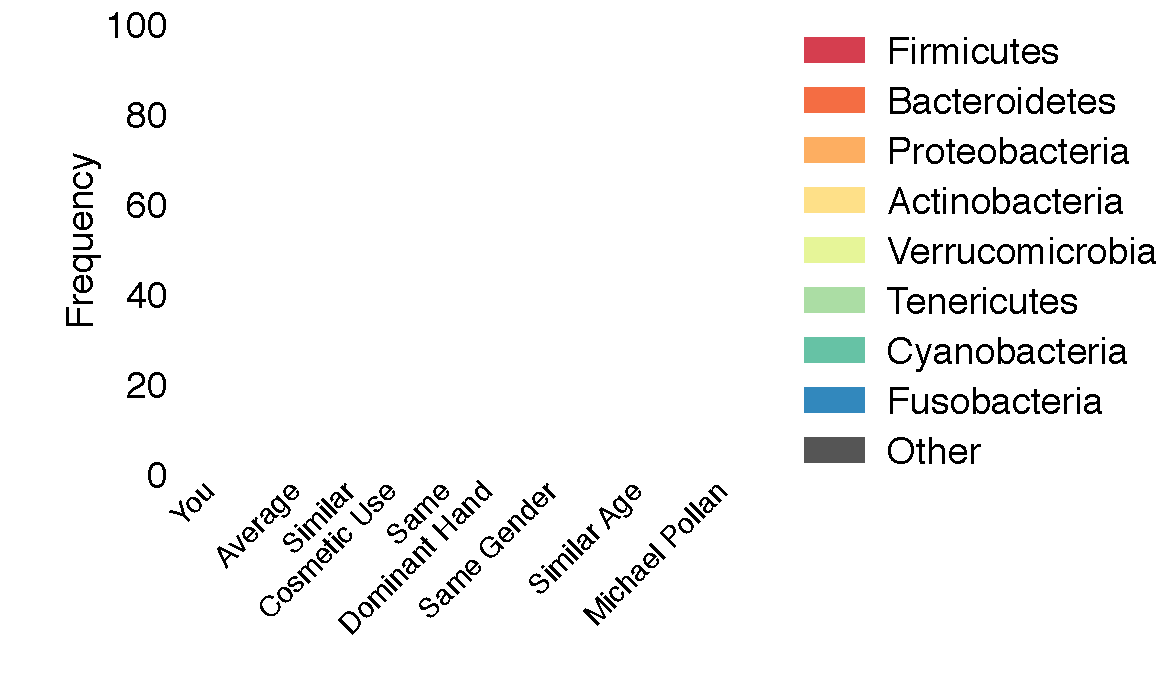
\includegraphics[width=3.65in]{statics/barchart_overlay_skin.pdf}}}{}
\end{overpic} 

&

\hspace{-5mm}
\raisebox{27mm}{
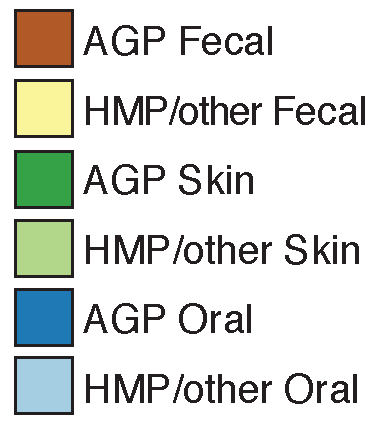
\includegraphics[scale=0.40]{pdfs-gut/figure1_legend.pdf}}
\hspace{-2mm}
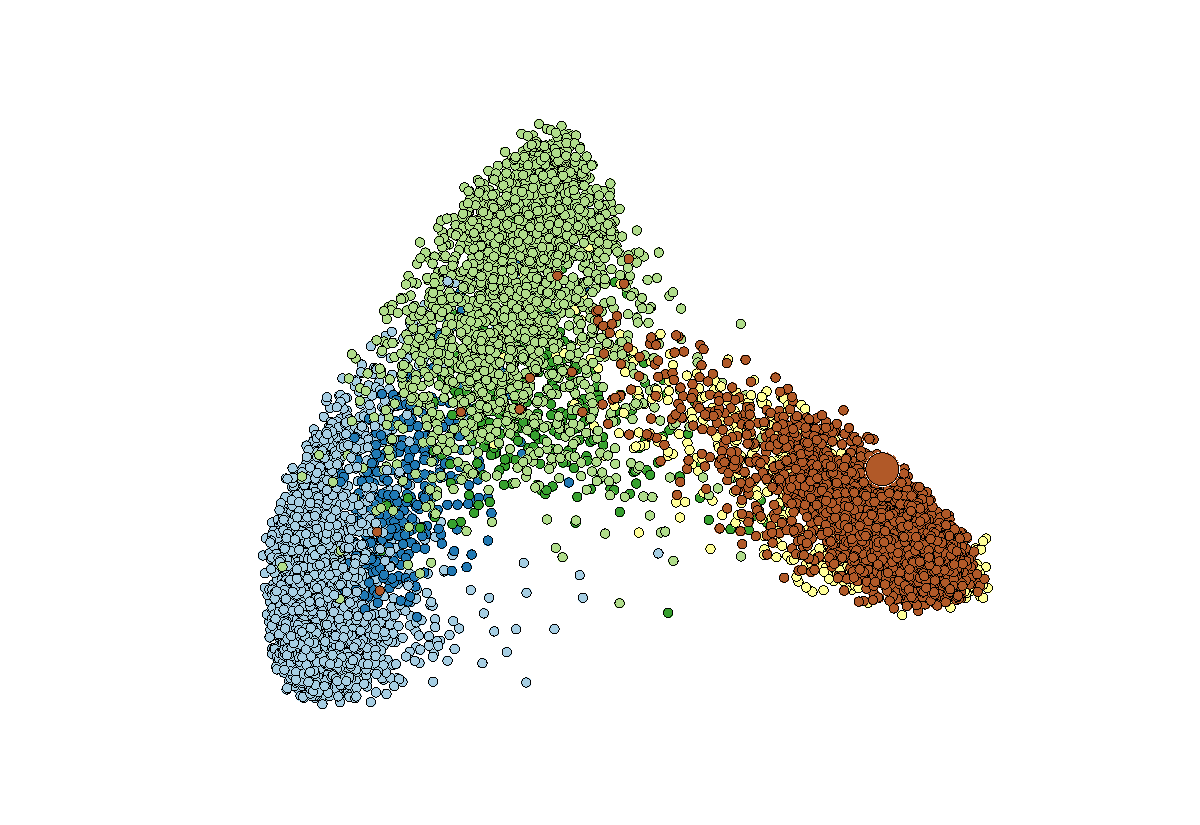
\includegraphics[scale=0.54, trim=3.5cm 1cm 2cm 2cm, clip=true]{figure1.pdf}

&

\hspace{5mm}
\ifthenelse{\equal{\sampletype}{oral}}{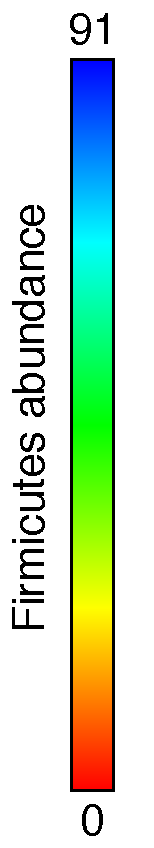
\includegraphics[scale=0.40]{statics/figure3_legend_firmicutes.pdf}}{}
\ifthenelse{\equal{\sampletype}{skin}}{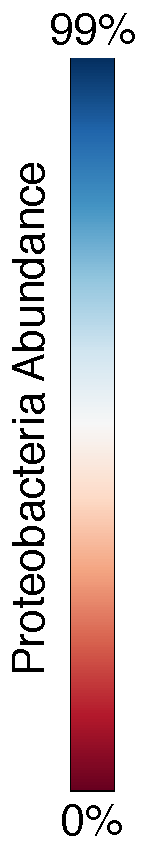
\includegraphics[scale=0.40]{statics/figure3_legend_proteobacteria.pdf}}{}
\hspace{-2mm}
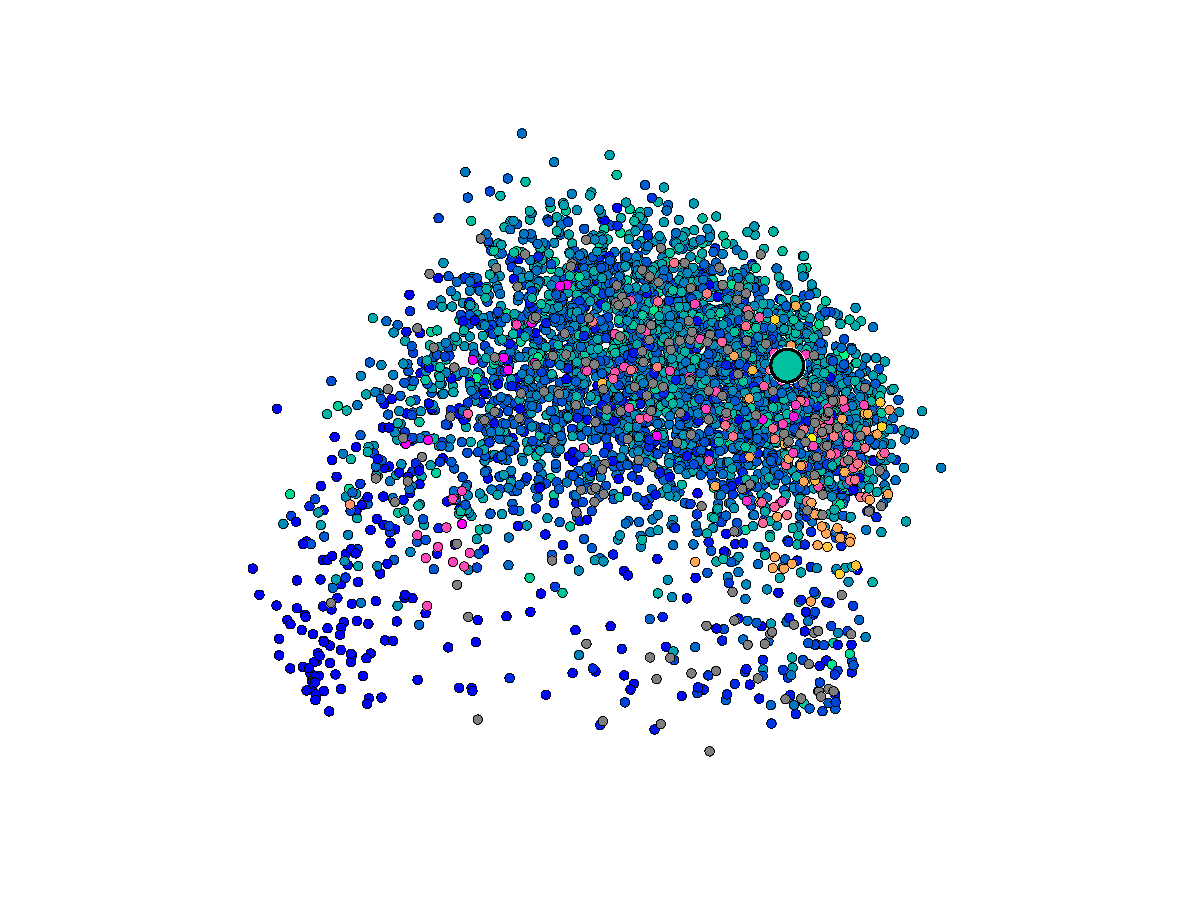
\includegraphics[scale=0.54, trim=3.5cm 1.5cm 2cm 1.5cm, clip=true]{figure3.pdf}


\\ \addlinespace[-2mm]

% captions - change makebox to framebox to see borders of captions

\hspace{9mm} \makebox[2in][c]{Different Subpopulations} \par 

& 

\hspace{20mm} \makebox[2in][c]{Different Body Sites} \par 

& 

\hspace{30mm} \makebox[2in][c]{The American Gut Population} \par

\end{tabular*}



\end{document}
